%!TEX root = thesis.tex

\chapter{Introduction}
\label{chap:introduction}

Robots play an increasingly important role in today's world because they enlighten human work in many different areas. Robots allow the automation of production processes but they are also utilized in other areas like medical surgery or even as household robots (autonomous vacuum cleaner, lawn mower, \ldots). Depending on the application domain, those robots require the ability to act in differing levels of autonomy. \citep{lavalle2006} describes the branch of \emph{robotics} as the area of automating mechanical systems that have sensing, actuation and computation capabilities. Part of the research in that branch is to create control software that allows to autonomously perform high-level tasks like grasping and object manipulation on robot hardware. The design and implementation of such high-level control software for a robot is a cumbersome task. The algorithms need to be tested and debugged during implementation process, but those tests come with a certain level of risk. Incorrect algorithms can lead to damages on robot components or their environment and entail costly repairs. In the worst case even people can get hurt by uncontrolled robot motions.\\

One solution to those problems is the usage of a simulator that physically models the robot and its behaviour as accurate as possible. Therefore it has to provide the same control interface to allow to test and debug each part of the software on the simulator before utilizing it on the real robot. Using a simulator allows to easily evaluate different design approaches and algorithms during the software development process. It can act as replacement for the real robot and facilitates parallelization of testing and debugging tasks, as the robot may be blocked by other persons or unavailable at certain times. It also allows to skip the technical overhead that often comes with working on the real device. Those considerations motivated the simulation part of the thesis. \\

The second part of the project focuses on robot motion planning. An autonomously acting robot needs to be able to plan the motions it needs to perform to fulfil a task. Moving the robot's hand for example cannot follow any arbitrary path towards a target pose. During that motion it might collide with itself or any other obstacle within its environment. That means those trajectories have to be planned and executed carefully to avoid accidental collisions and to generate smooth and well controlled motions with respect to the limits of the robot. The resulting trajectories should be preferably short and may not contain unnecessary motions. 


TODO: Complete the introduction!!! The project targets are specified in the following section.


%Therefore it needs to be able to move towards target positions without colliding with obstacles in its environment. Research in the branch of robotics tends to enable robots to perform certain tasks largely autonomous. Without motion planning the motions have to be constantly specified by a human operator - not preferable, only suitable for repetitive tasks.

\section{The IIS-Lab Robot setup}
\begin{figure}[ht]
	\centering
  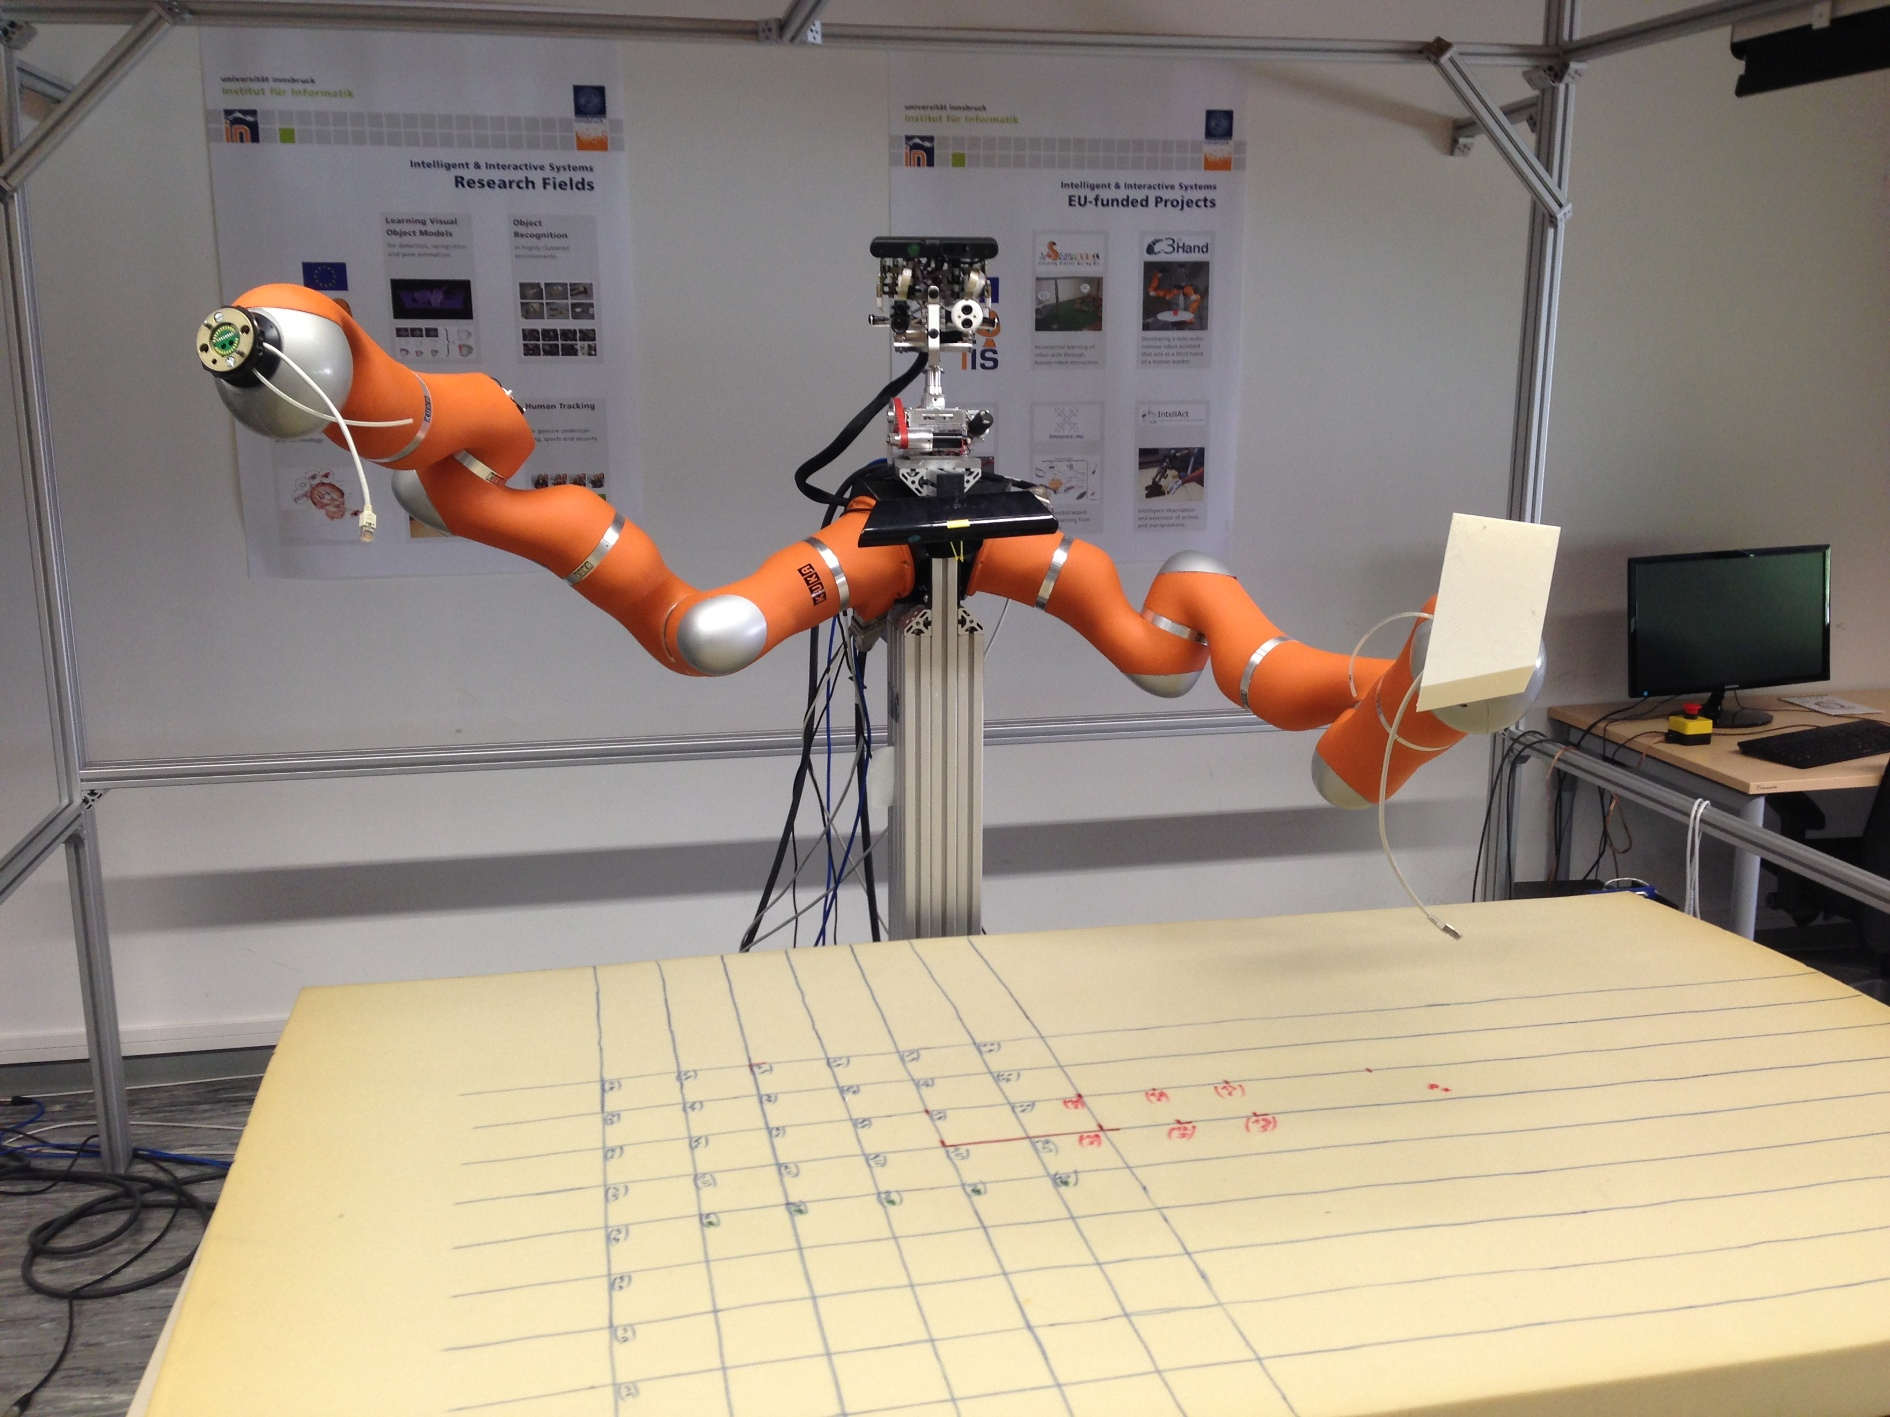
\includegraphics[width=0.75\textwidth]{images/robot_setup.jpg}
	\caption{Current setup in the IIS-Lab}
	\label{fig:iis_setup}
\end{figure}

The structure of the robot setup in the IIS-lab changes frequently, as new robot components are introduced and arrangements are modified. The setting considered within this thesis is a snapshot though the solutions that will be developed should be customizable to reflect alternating settings. The main part of the robot setup consists of an aluminium torso with two mounted 7 DOF\footnote{Degrees of freedom - the number of independent variables, necessary to describe a robot's configuration} KUKA LWR4+ \citep{kuka2012} robot arms, as shown in Figure \ref{fig:iis_setup}. The IIS-Lab also owns two Schunk SDH-2 \citep{schunk2010} robot hands that can be mounted to the robot arms for grasping experiments. The workspace where those experiments usually take place is the table in front of the robot which is covered with a foam mat for security reasons. Additionally there is a Kinect camera mounted on the robot torso, between both arms. A Kinect camera contains a vision sensor and a depth sensor. The vision sensor provides RBG images of the task environment. The depth sensor returns depth images where each pixel represents the distance to its corresponding point in the world \citep{andersen2012}. Control and data exchange with all available components is based on the robot operating system ROS which will be described in the next section.

\section{The Robot Operating System (ROS)}

The implementation of the project requirements is based on ROS. Therefore a brief introduction about the basic concepts\footnote{http://wiki.ros.org/ROS/Concepts} shall be given here. The explained terminology will be used throughout this thesis. As stated in \cite{quigley2009}, ROS is not an operating system in the classical sense. It runs on top of a host operating system (usually linux) and can be seen as an additional communication layer, providing various mechanisms for inter-process communication. A ROS system consists of a number of \emph{nodes}. Each node is an independent computation unit that runs in its own process, adding clearly defined functionality to the overall system. For example one node can be responsible for planning, another one for perception and a third one for controlling the hardware. Nodes communicate to each other by passing \emph{messages}, using the ROS communication infrastructure. Messages are strictly typed data structures, defined in a special message composition format\footnote{http://wiki.ros.org/msg}. They can be composed of primitive types like float, integer or string, but also of other message types. Therefore it is possible to create arbitrarily complex messages for each use case. \\

Messages are published to \emph{topics}. A topic is a strongly typed message bus, addressed by its name. Arbitrary nodes can connect to a topic in parallel, as long as they use the correct message type. Each node can publish and subscribe to a number of topics. It is also possible that various nodes publish to the same topic. Topic names are strings, used to identify topics. They can be organized into namespaces to build a tree hierarchy comparable to the directory structure in a file system. This is very important, as for example the simulator should use similar topic names as the real robot. The namespace concept allows both instances to use identical names but each one in its own namespace. The following samples represent valid topic names:
\begin{itemize}
\item \texttt{/} (this is the root namespace)
\item \texttt{/component/topic}
\item \texttt{/simulation/component/topic}
\item \texttt{/real/component/topic}
\end{itemize}

The topic names used in the current project follow the IIS lab internal naming conventions. Each topic name has the structure
\begin{center}
\texttt{/[namespace]/[component name]/[control type]/[name]}
\end{center}
The namespace is necessary to distinguish between the topics of simulator and real robot. All simulator related topics reside in the \path{simulation} namespace. The component name identifies a specific robot component within that namespace, e.g. \texttt{left\_arm} or \texttt{right\_sdh}. The control type groups sets of topics into different categories. Possible values are \texttt{joint\_control}, \texttt{cartesian\_control}, \texttt{sensoring} and \texttt{settings}. Finally, the chosen name is used to identify the specific topic within that category. For example the topic \path{/simulation/left_arm/joint_control/move} states a topic named \path{move} in the category \path{joint_control} for a simulated component, named \path{left_arm}. \\

\begin{figure}[h]
	\centering
  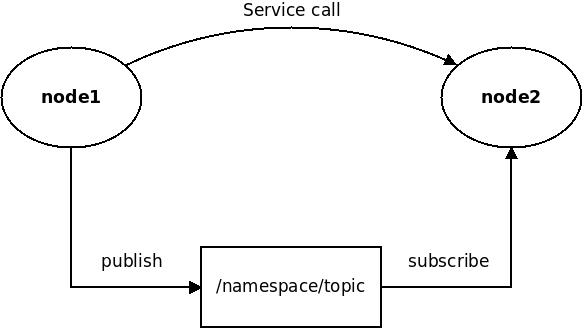
\includegraphics[width=0.5\textwidth]{images/ros_concept.jpg}
	\caption{ROS nodes, topics and services}
	\label{fig:ros_concept}
\end{figure}

The communication via ROS topics is asynchronous - involved nodes may even not be aware of each others existence. Synchronous message exchange between nodes happens via ROS \emph{services}. In contrast to topics, a service with a given name can only be offered by one single node. Services are addressed, using the same naming strategy as topics. The service message is composed of a request and a response part. A client node that sends a service request will block, until the advertising node has handled the request and delivers a response. The concepts of ROS topics and services are shown in Figure \ref{fig:ros_concept}.\\

The nodes of a ROS system can be distributed over various different machines. One of them has to be the dedicated \emph{ROS master}. The master is responsible to handle topic and service registrations and holds information about the involved ROS nodes. Other machines connect to the master via network. The ROS master also provides a centralized \emph{parameter server}. This is a shared dictionary that can be used to store and retrieve configuration data and other shared parameters. Nodes can access the parameter server at runtime and read or modify its content. \\

A system usually consists of a large number of nodes that have to be configured and started. This startup process can be automated, using so called \emph{launch files}. Those are simple textfiles, holding startup information and configuration details for one or more nodes in an XML like syntax\footnote{http://wiki.ros.org/roslaunch/XML}. Using the \emph{roslaunch} command line tool, a whole system of nodes can be configured and launched at once. \\

ROS is a modular software system organized into \emph{packages}. Each package adds clearly defined functionality and can be reused in other systems. Custom functionality is added to a ROS system by creating a new package and developing the required piece of software. A package might contain one or more ROS nodes or even only configuration data. Existing packages are usually installed, using a software repository package manager. A very useful ROS package is the visualization tool \emph{RViz}. This tool provides a number of different plugins that allow to display robot setups and configurations, planned trajectories or image data from a vision sensor. RViz gets utilized in the motion planning related part of this project.

\section{Project Targets}

The first goal of this project is to create a realistic replication of the IIS-Lab robot setup, using a suitable simulation platform. The solution needs to be able to generate proper sensor data and provide the same ROS control interface as the real robot. Additionally it would be preferable that the solution is able to detect and visualize accidental collisions of robot components with the environment. The necessary steps are explained in Chapter \ref{chap:simulation}.\\

The second objective is to choose and integrate a state of the art motion planning framework into the existing setup. The required functionality includes solving inverse kinematics\footnote{Problem of finding possible joint settings for the robot to achieve a desired end effector position and orientation in Cartesian space \citep{craig2005}} (IK) problems and planning collision-free trajectories for complex robot motions in joint space and Cartesian space. This integration process is described in Chapter \ref{chap:moveit}. \\

The proper functioning of the planning framework will then be shown by planning and executing a benchmark pick and place task as explained in Chapter \ref{chap:pick_place}. That chapter starts with an overview about grasping tasks in general and explains the resulting planning problems in detail. After that it will be shown how those planning problems can be solved using the planning framework and how the resulting motion plans are executed on the simulated or real device.\\

The implementation of those objectives requires to determine the kinematic, dynamic and volumetric properties of the involved robot components. This includes to do an exact measuring of the existing robot setup in the IIS-Lab and determine the placement of the involved components relative to each other to be able to create an internal representation of the world. 

%For Cartesian positioning functionality it is also necessary to define a world reference frame and place components relative to that reference frame. \citep{craig2005} describes the inverse kinematics (IK) problem as the problem of finding possible joint settings for the robot to achieve a desired end effector position and orientation in Cartesian space. Forward kinematics (FK) is the reverse problem of finding the position and orientation of the end effector, given a set of joint angles. The end effector is the tool, mounted on the tip of the robot arm.
